\subsection{Tool plate} %Ande

In the old design the battery box which sticks out from the main hull is visible, see the fig. \ref{Toolplate}. The new design has a bigger tool plate that encloses the battery box, see fig. \ref{toolplate2}. There are also room for two markers, a gripper, a pneumatic box, a temperature sensor and a pressure sensor.

	\begin{figure}[!ht]
	\begin{center}
		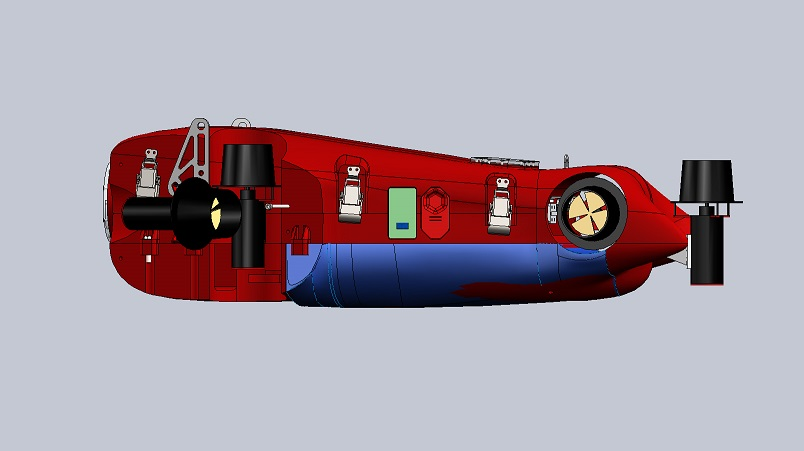
\includegraphics[width=100mm]{./Images/Mechanics/Naiadassembly2.JPG}
		\caption{The new toolplate make battery box invisible}
		\label{toolplate2}
	\end{center}
\end{figure}

The redesigning of tool plate was dependent on the gripper and pneumatic design. Since it was decided to make a new gripper rater than the suggested one and this new gripper did not have a design, it was difficult to redesign and manufacture the tool plate.

The solution was to make a modular design which is independent of the equipment's design. The new design is a plate with several holes which can be attached to the main hull by screws. The tool plate have then been divided into several parts each equipment have it's own part. Each part will then be attach to the tool plate by screwing it too the tool plate holes.  

	\begin{figure}[!ht]
	\begin{center}
		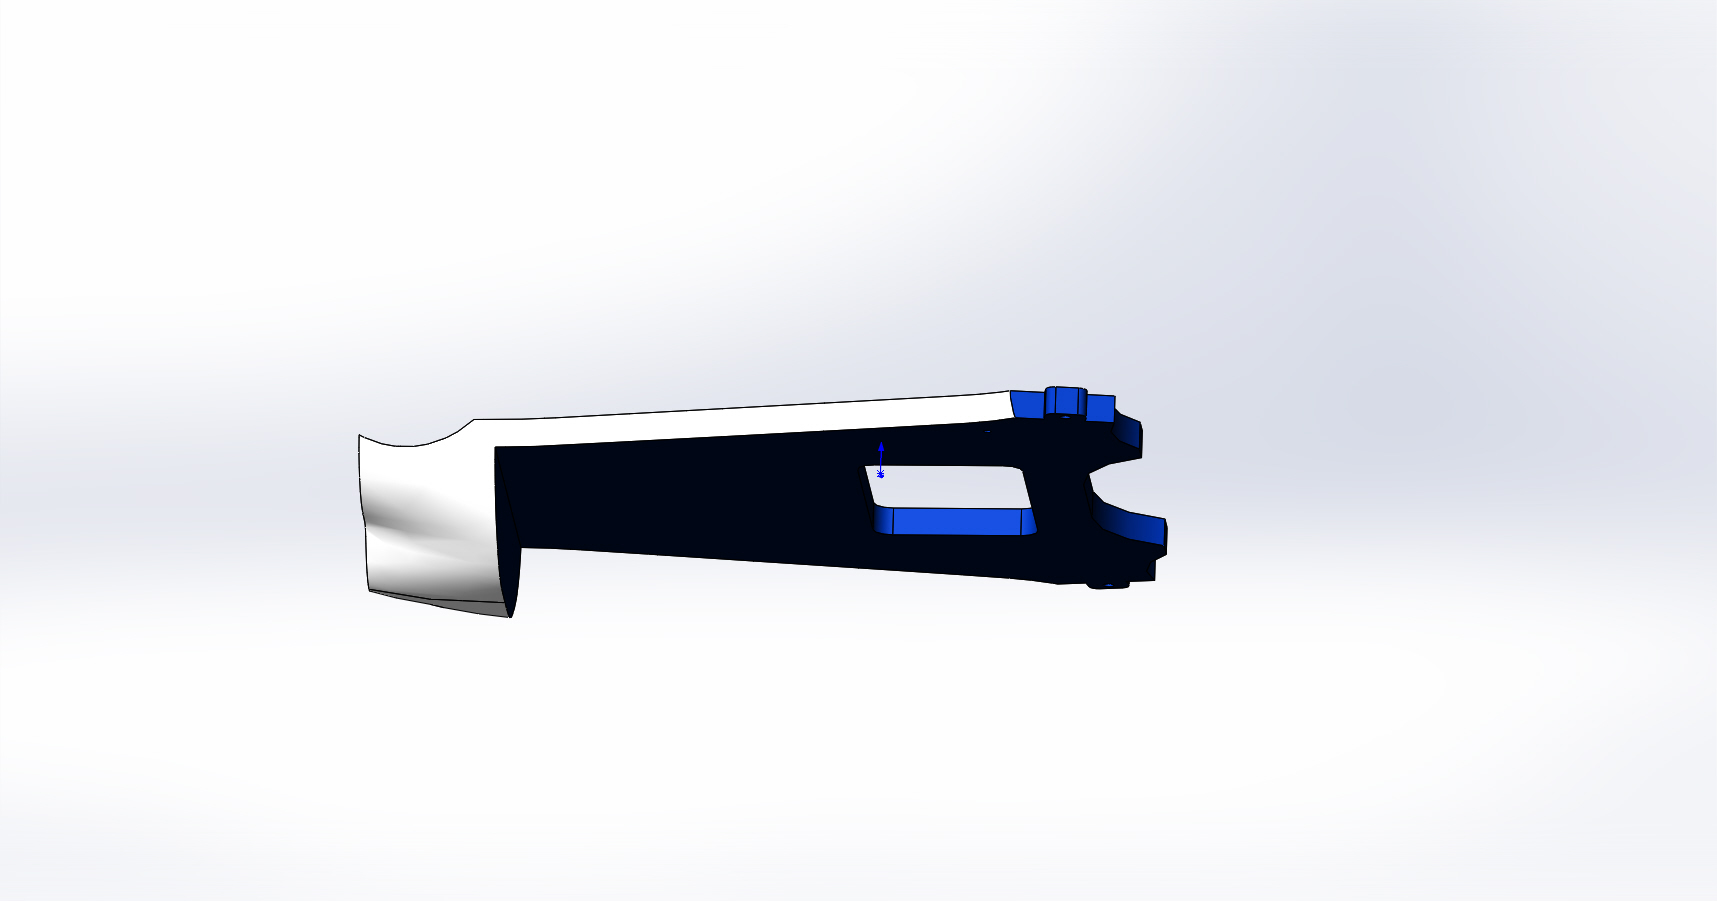
\includegraphics[width=100mm]{./Images/Mechanics/PlateTool.JPG}
		\caption{The new design of a modular tool plate}
		\label{hyrdrobox}
	\end{center}
	\end{figure}
	
	\subsubsection{Pneumatics}
In the beginning it was decided to use pneumatic system to operate the markers, the torpedoes and the gripper. Since the new gripper is considered to not use the pneumatic system to operate anymore, it was suggested that the marker and the torpedo could use solenoids instead, this is much less complicated. Therefor for future work it is recommended to look into if the torpedoes could work with solenoid instead. The biggest worry in using a solenoid to operate torpedoes is the space in the front tool plate.

	\subsubsection{Sensors}
Naiad is equipped with a pressure sensor and it is also supposed to have a temperature sensor. Both sensors will be placed in the back of the tool plate. Where the sensors will be attach to are not designed yet. Since Naiad uses a modular tool plate, a box will be designed were both sensors will be attached. The box will then be screwed to the tool plate.
	
	\subsubsection{Markers} %Martina
	\label{Markerss}
	\noindent The markers should preferably be placed near a camera so the system can detect the target for the marker. There are two camera systems, one facing forward and one facing downwards. As the markers are supposed to fall downwards, this leaves one camera system to place the markers near. They can be placed in front of or behind the bottom camera housing. The markers are placed between the front tool plate and the bottom camera housing. This space is limited, but as the back of the tool plate is crowded this placement seemed like a good choice.
